\chapter{Representation of the Memory of an Energy Cube Organism (1966)}

The energy cube organism is a conscious organism which is nothing but 
energy confined to a cubical space. It rests on a rectangular energy slab, in a 
stationary, colorless liquid, separated from the slab by a thin film of liquid. 
It has been on the slab for an indefinitely long time. There are in fact two 
infinite bodies of the liquid, alternating with two infinite empty spaces; the 
four volumes are outlined by two intersecting planes which just miss being 
perpendicular. The slab is poised, at a slant, on the faces of the upper body 
of liquid, near where they meet. There are no other objects in the bodies of 
liquid. The slab, liquid, and spaces are the energy cube organism's entire 
cosmology. (See figure \ref{energycube}.)

\begin{figure}
\centering
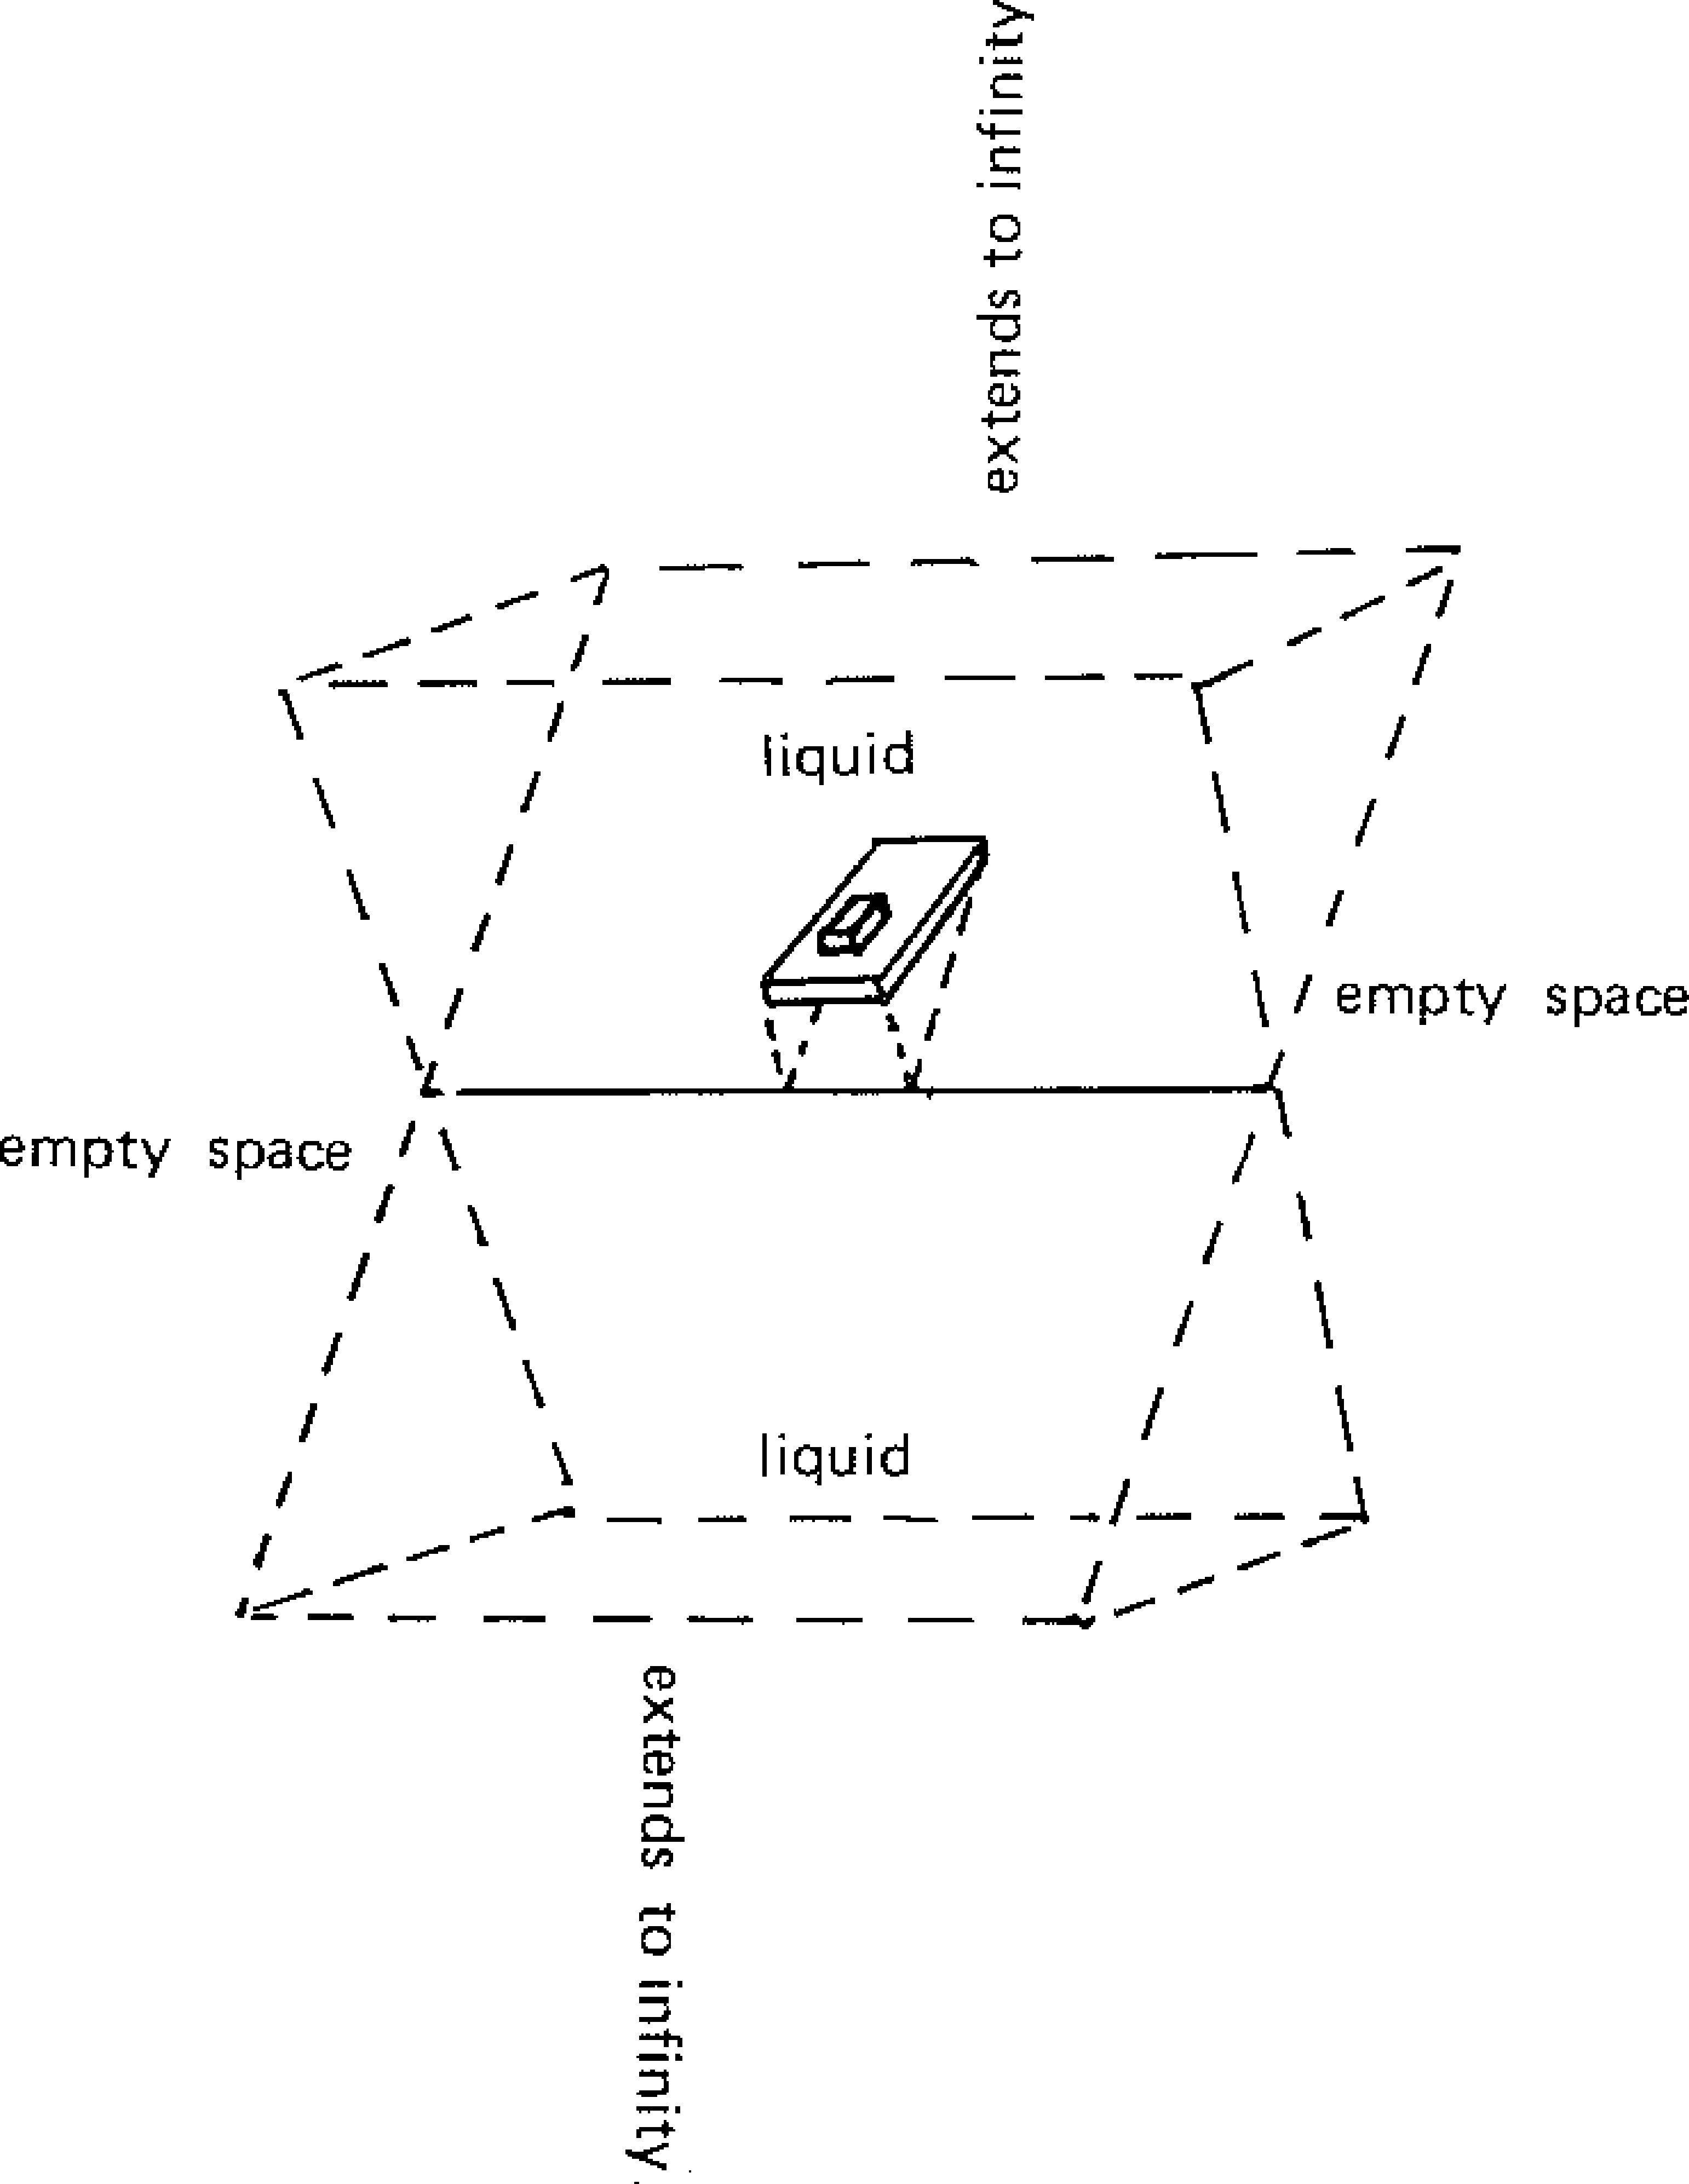
\includegraphics[width=3.75in]{img/energycube}
\caption{tktk}
\label{energycube}
\end{figure}

The energy cube organism can continuously change position, 
continuously and instantly moving the liquid from its path into its wake so 
as to make no current in the liquid. For almost as long as it has been on the 
slab, the organism has devoted itself to crossing the slab, from the slab's edge 
on one face of the liquid to its edge on the other. 

The energy cube organism has a conscious memory (by which I mean 
strictly a memory of what it did and what happened to it, the past events of 
its existence). The memory consists of symbols which are given \enquote{meaning} 
by their extra-linguistic mental associations---in human terms, it consists of 
language. The complete memory contains tens of thousands of partial 
memories, which the organism can only have one at a time. Going through 
the partials---which it does as if they were the phonemes of one long 
word---constitutes its one complete memory. Each partial is a memory of the 
difference in the organism's minimum distances from the destination edge, at 
the beginning, and at the end, of some interval of time. Call the difference its 
\enquote{progress.} The total of time intervals in all the partials completely covers 
the interval from the earliest remembered event to the most recent 
remembered event. As time passes, more partials are added to the complete 
memory. The production of partial memories is an involuntary process of 
the organism. 

The memory is temporally dual. The interval for each partial is an 
interval of fixed time, defined by its duration, and the distance from the 
fixed time when the energy cube organism appeared on the slab up to the 
interval's end. But it is also a sliding interval, defined by its duration, and a 
constant distance from the present instant back to the interval's end. When 
partials are added to the memory, each of the former intervals exactly covers 
the tire not already covered, up to the absolute time when the partial is 
added. But the latter intervals, while they never overlap, can have gaps 
between them. The intervals generally are of different durations. The energy 
cube organism lacks any independent extra-linguistic memory, any mental 
reliving of the past, which could conflict with the dual temporal memory. 
There is no form to the past other than that of the memory's language. (See 
figure \ref{ecubegraph}.)

The order of the partials in the complete memory is a linguistic 
phenomenon which indicates the method the organism has been using to 
move itself---and thus the order (with its extra-linguistic associations) is the 
memory of the method. A single method is everything to be done by the 
energy cube organism to move itself, throughout the entire time it takes to 
reach the destination edge. There are different possible methods, and each 
could get the organism across; but the methods cannot be combined in any 
way. Every order of all partials signifies a different possible method. These 
possible methods are in no special order. When a partial is added to the 
memory, the number of possible methods is increased by a factor equal to 
the new number of partials. 

\begin{figure}
\centering
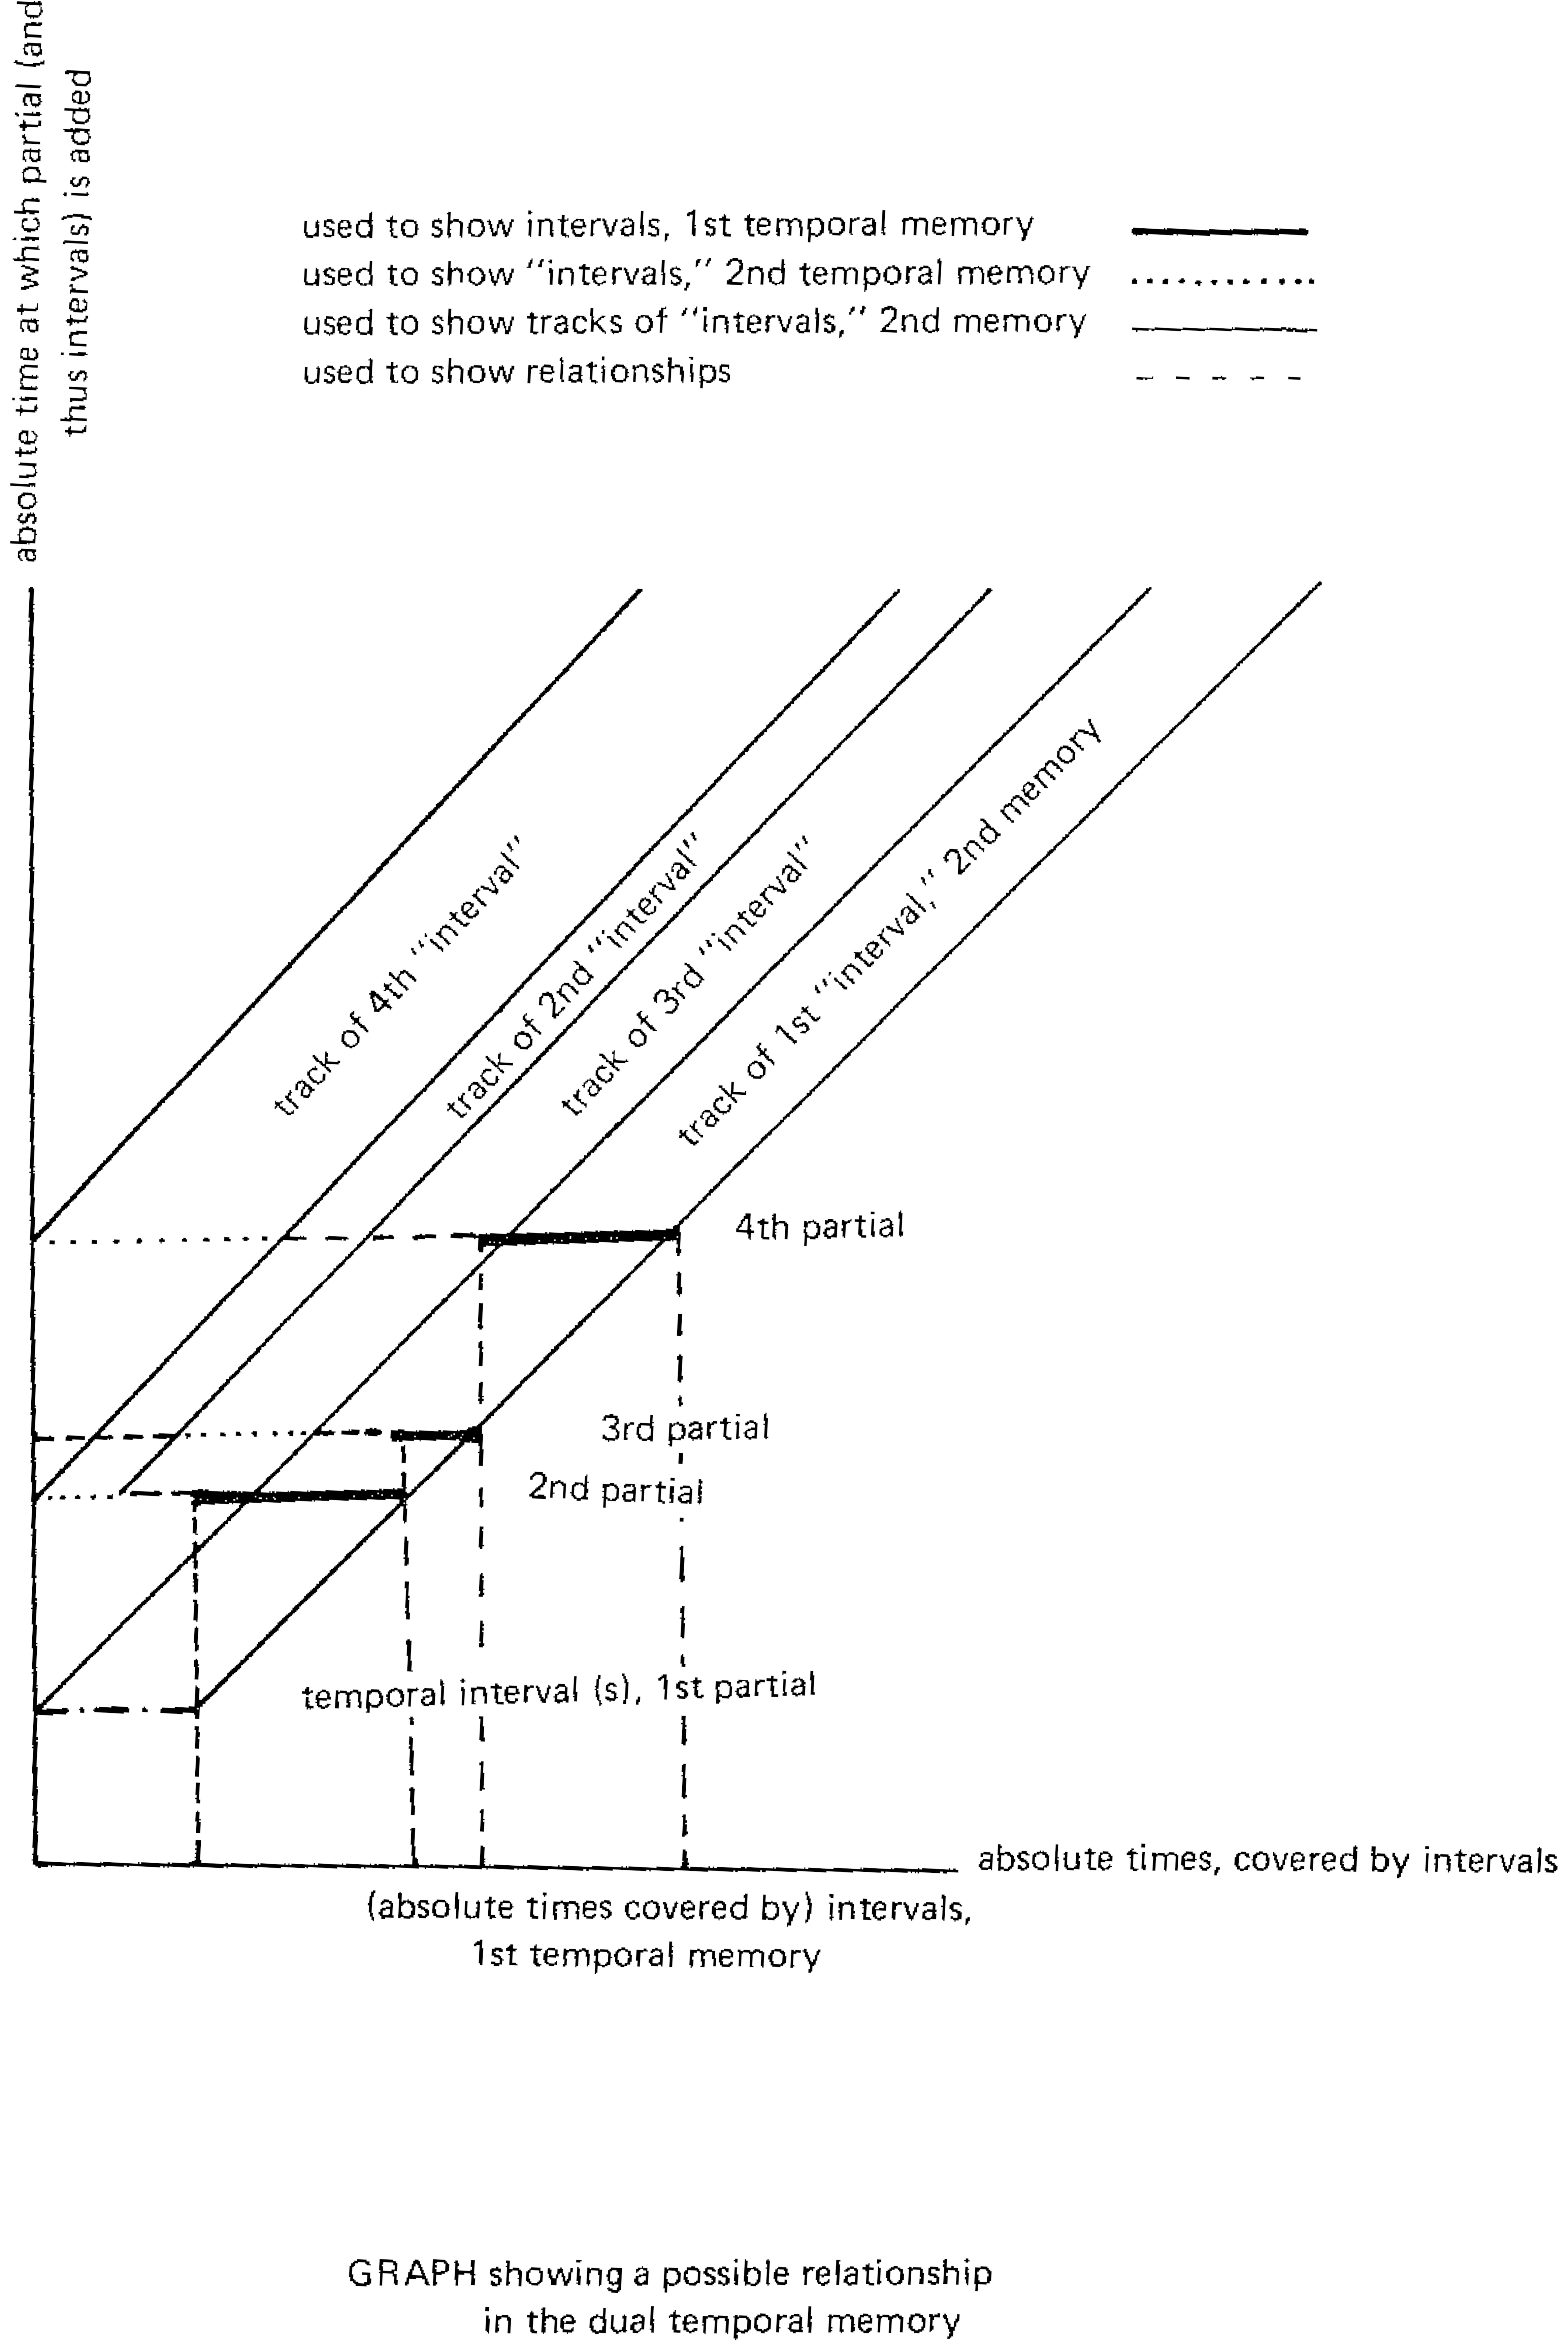
\includegraphics[width=4in]{img/energycubegraph}
\caption{Graph showing a possible relationship in the dual temporal memory.}
\label{ecubegraph}
\end{figure}


Now the complete memory is obtained by going through the partials---in 
any order! Any order gives the memory. This feature, which can be 
precisely characterized in terms of the memory language, is perhaps the most 
remarkable feature of the whole cosmology. An approach to this feature in 
human terms is to say that when the organism goes through the partials, (it 
dreams that) it has been using the method indicated---and is presently using 
it. It (does not remember the dream, and) does not remember going through 
the partials. It has no other memory of which method it has been using. 

The organism moves itself by mental exertion, teleports itself. The 
\enquote{possible methods} are mental routines. These routines draw on the 
following standard mental resources. The organism can assume at will many 
\enquote{mental states.} By \enquote{mental state} I refer to a mental \enquote{stage} or \enquote{space} or 
\enquote{mood} in which visualizing, remembering, and all imaging can be carried 
on. Some human mental states are general euphoria, stupor, general anxiety, 
dreaming, dizziness, empathy with another person, and clearheadedness, the 
normal state in which work is performed. These states are not defined by 
specific imagings, but are \enquote{spaces} in which imaging is carried on. The 
organism changes its state by changing from one form of energy to another, 
gravity, magnetism, electric energy, radiated heat, or light. In these states, 
the organism has an unlimited capacity to image; in human terms, to 
visualize. There are visualized regions of colored liquids. Call them \enquote{fluid 
colors.} There are visualized glowing surfaces, and there are black regions or 
\enquote{holes.} There are visualized \enquote{covers,} \enquote{lattices,} and \enquote{shells,} which are all 
formed from transparent planes, spherical surfaces and the like. Call them 
\enquote{orojected surfaces.} The fluid colors can be stationary or flowing. There are 
\enquote{channels,} which are strung-out series of fluid colors. There are 
\enquote{reservoirs,} which are clusters of fluid colors. A channel can be closed or 
open. Two channels can cross each other. There are pairs of channels such 
that earlier members of each channel flow into later members of the 
other---called \enquote{screw-connected} channels. Fluid colors often occur on or 
within projected surfaces. Projected surfaces can be growing or held. A 
visualization can be at the forefront of attention, or in the back of the mind. 
That is, states have depth, and visualizations can be at different depths. The 
state as a whole can be \enquote{frozen} or \enquote{melted.} A human approach is to say 
that a \enquote{frozen} state is set or fixed; while a \enquote{melted} state is fluid---the state 
itself flows. A state can be projected into \enquote{superstate,} gaining an abnormal 
amount of mental energy and becoming superdizziness or superanxiety, for 
instance. 

Most interesting, states in different possible methods can have contact 
with each other. A human approach is to say that dreams are so flexible that 
the organism can dream that an actual state is\slash was in contact with a state in 
a possible method. One sort of cross-method contact is for states to be 
\enquote{interfrozen}---more easily frozen because they are somehow mixed. They 
can also be \enquote{intermelted.} 

I will describe a method, as the organism would be conscious of it in 
remembering. For concreteness, I will refer to the different states with the 
names of human states rather than with letters. Channels are generated in a 
frozen stupor, and become fixed at the forefront of attention of euphoria 
intermelted with a possible state. The screw-crossed channels erode crevices 
in a held lattice, which breaks into growing sheets (a variety of covers). The 
sheets are stacked, and held in a frozen dream thawed at intervals for 
reshuffling of the stack. The dream becomes melted, and proceeds in a 
trajectory which shears, and closes, open channels. If no violation of the 
channels cross-mars the melt, the stack meshes with the sharp-open channels. 
The dream becomes interfrozen, and mixed clear-headed states compress the 
closed channels which were not fixed at the dream's surface. A fused 
exterior double-flash (a certain maximally \enquote{glowing surface}) is 
expand-enveloped by euphoria, which becomes dizziness; and oblique 
lattices are projected from the paralinear deviation of guided open channels 
in it. Growing shells are dreamed into violet sound-slices (certain synesthetic 
\enquote{fluid colors}) by the needed jumped drag (a generic state), a crossfrozen 
dream. Channels in a growing anxiety enspiral concentric shells having 
intermixed reservoirs between them, during cyclic intersection of the anxiety 
in superstate. And on and on. Time is here the time it takes to carry out the 
successive steps of the routine. 

The energy cube organism language, the symbols constituting the 
partials, are themselves mental entities. A partial is a rectangular plane 
glowing surface, which has two stationary plane reservoirs on it, and has a 
triangular hole in it. As a mental entity, in other words, a partial is a 
visualization like those which are part of the methods. The perimeter of the 
triangular hole equals the organism's progress in the corresponding time 
interval. Absence of the hole indicates zero progress. 

The fluid colors in each of the reservoirs on each partial memory are 
primary colors, and are mixed together. Speaking as accurately as possible in 
human terms, in each reservoir there is precisely one point of \enquote{maximum 
mixture} of the primary colors. The primary colors are mentally mixed in 
any way until the right amount of mixture is reached. There is a scale of 
measurement for amounts of mixture of the colors. There is a scale for 
vertical distances on the surface---for how far one point is below another. The 
difference in amounts of mixture at the two points of maximum mixture 
corresponds to the length of the first temporal interval; and the difference 
between the maximum possible amount of mixture and the lesser of the two 
amounts of maximum mixture on the surface corresponds to the distance 
from the fixed beginning time to the interval's and. The vertical distance 
between the two points of maximum mixture corresponds to the length of 
the second temporal interval; and the vertical distance from the middle of 
the surface to the point nearer it corresponds to the constant distance from 
the present instant back to the interval's enc. The middle of the surface 
represents the present, and the upper half represents the future; the 
reservoirs are all in the lower half. For each partial it is necessary to 
determine (1) the number of units of duration per unit difference in 
amounts of mixture; and (2) the number of units of duration per unit 
difference in vertical distances. The average glow per unit area of each 
glowing surface (excepting the hole) is correlated with a pair of numbers 
constituting this information. 

Finally, turning all the partial memories upside down---and reflecting the 
first temporal memory in the present instant, so that the intervals' absolute 
distances from the present are preserved---gives the precognition of the 
organism's future course of action, tells what progress will be made when 
and by which method. 


\section*{The Representation}

This essay accompanies a representation of the energy cube organism's 
memory ---hence its title. The way to picture the memory, naturally, is to 
make something that looks like the partials. I have represented the partials 
by rectangular sheets of paper of different translucencies with mixtures of 
inks of primary colors on them and holes cut in them; together in an 
envelope, which bears the injunction not to have more than one sheet out at 
a time. Three of the tens of thousands of partials are represented. 
